\documentclass[preliminary]{eptcs}
\providecommand{\event}{WORDS 2011} \usepackage{breakurl}             


\usepackage[utf8]{inputenc}
\usepackage{tikz}
\usetikzlibrary{automata}
\usepackage{amssymb}
\usepackage{amsmath}
\usepackage{cancel}

\author{Thierry Monteil
\institute{CNRS -- Université Montpellier 2\\
\burl{http://www.lirmm.fr/~monteil}}
}


\def\titlerunning{The complexity of tangent words}
\def\authorrunning{Thierry Monteil}



\newtheorem{Theorem}{Theorem}
\newtheorem{Corollary}[Theorem]{Corollary}
\newtheorem{proposition}[Theorem]{Proposition}
\newenvironment{proof}{\noindent {\bf Proof:}}{\hfill  \\}




\title{The complexity of tangent words}


\date{}

\begin{document}

\newcommand{\qed}{\hfill }

\maketitle


\begin{abstract}
In \cite{MonteilDGCI2011}, we described the set of words that appear in
the coding of smooth (resp. analytic) curves at arbitrary small scale. The
aim of this paper is to compute the complexity of those languages.
\newline \newline
\emph{Keywords:} Cutting sequence, symbolic coding, word complexity,
multigrid convergence, Sturmian word.
\end{abstract}


\section{Introduction}


A \emph{smooth curve} is a map  from a compact interval  of the
real line to the plane, which is  and such that  for any  (this last property is called \emph{regularity}).
Any such curve can (and will be considered to) be arc-length
reparametrised (\emph{i.e.} ).
\newline
We can approximate such a curve by drawing a square grid of mesh  on
the plane, and look at the sequence of squares that the curve meets.
For a generic position of the grid, the curve  does not hit any
corner and crosses the grid transversally, hence the curve passes from a
square to a square that is located either \emph{r}ight, \emph{u}p,
\emph{l}eft or \emph{d}own of it.
We record this sequence of moves and define the \emph{cutting sequence} of
the curve  with respect to this grid as a word  on the alphabet 

which tracks the lines of the grid crossed by the curve .
\newline
The following picture shows a curve  with cutting sequence
.
\begin{center}

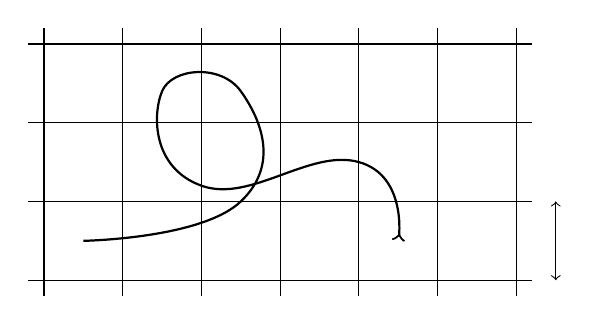
\begin{tikzpicture}
    \draw[step=1,thin] (0,0) +(-0.2,-0.2) grid +(6.2,3.2);
    \draw[<->] (6.5,0) -- (6.5,1);
    \draw[right] (6.5,0.5) node {};
    \draw[-<,thick] plot[smooth,tension=0.9] coordinates{(0.5,0.5) (2.5,1) (2.5,2.4) (1.5,2.4) (2,1.2) (4,1.5) (4.5,0.5) }; 
    \draw[thick] (4.5,1.5) node {\bf };
\end{tikzpicture}

\end{center}
Note that since the grid can be translated, a given curve may have more
than one cutting sequence for a given mesh .
Our knowledge of the curve from one of its cutting sequences increases
when the mesh  decreases, and when the mesh approaches , the local
patterns of the cutting sequence play the role of discrete tangents. Such
words are called \emph{tangent words}, their first properties were
described in \cite{MonteilDGCI2011}.
Cutting sequences associated to straight segments are known to be exactly
the \emph{balanced words}, which are also the finite factors of Sturmian
words.
It turns out that the tangent words strictly contain balanced words, and
that -balanced words strictly contain tangent words. The aim of this
note is to count the number of tangent words (resp. tangent analytic
words) of a given length, in order to quantify those inclusions.






\section{Tangent words}
Tangent words are the finite words that appear in the cutting sequences of
some smooth curve for arbitrary small scale.
More precisely, let  denote the set of factors of the cutting
sequence of the curve  with respect to the square grid  (when
the curve hits a corner, the cutting sequence is not defined and we set
).
We define the \emph{asymptotic language} of  by

More generally, when  is a set of curves, let us denote by  the
set . When  is the set of smooth
curves, we denote  by , and call its elements
\emph{tangent words}. When  is the set of analytic curves, we denote
 by , and call its elements \emph{analytic tangent words}.
The two languages  and  are factorial and extendable.
\newline \newline
For the sake of simplicity, we will focus on curves going right and up,
\emph{i.e.} smooth curves such that both coordinates of  are
positive for any . Let us rename  and  by  and 
respectively to stick to the usual notation about binary words.
\newline \newline
The following results are proved in \cite{MonteilDGCI2011}.

\subsection{Combinatorial characterisation (desubstitution)}

Balanced words are know to have a hierarchical structure, where the
morphisms  and  play a crucial role \cite{PytheasFogg2002}
\cite{Lothaire2002}.
The same renormalisation applies to tangent words.
\newline
Given a finite word , we can ``desubstitute'' it by 
\begin{itemize}
\item removing one  per run of  if  does not appear in , or
\item removing one  per run of  if  does not appear in .
\end{itemize}
This desubstitution map (denoted by ) consists in removing one
letter per run of the non-isolated letter. An accelerated version of this
desubstitution consists in removing a run equal to the length of the
shortest inner run from any run of the non-isolated letter (including
possible leading and trailing runs even if they have shorter length). 
\newline
If we repeat this process as much as possible, we get a \emph{derivated
word} denoted by . The word  is balanced if, and only if, 
is the empty word, and the derivation process is related to the continued
fraction development of the slope of the associated straight segment.


A word is said to be \emph{diagonal} if it is recognised by the following
automaton with three states, which are all considered as initial and
accepting: 
\begin{center}
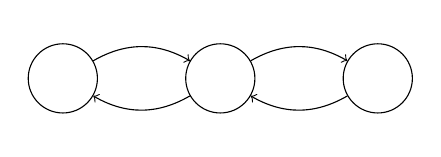
\begin{tikzpicture} \node[state] (Q) {}; \node[state] (R) at (2,0) {};
\node[state] (S) at (4,0) {}; \path[->] (Q) edge [bend left]  node [above]
{} (R); \path[->] (R) edge [bend left] node [below] {} (Q);
\path[->] (R) edge [bend left]  node [above] {} (S); \path[->] (S) edge
[bend left] node [below] {} (R); \end{tikzpicture}
\end{center}


A word is said to be \emph{thin diagonal} if it is diagonal and only two
states are visited during its recognition.



A word is said to be \emph{non-oscillating diagonal} if it is recognised
by the following automaton with eight states, which are all considered as
initial and accepting:
\begin{center}
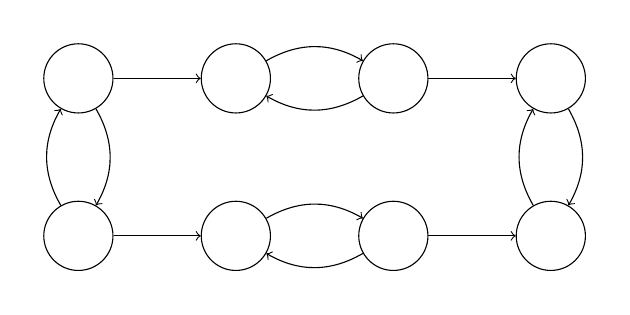
\begin{tikzpicture}
\node[state] (R) at (2,0) {};
    \node[state] (S) at (4,0) {};
    \node[state] (T) at (6,0) {};
    \node[state] (U) at (8,0) {};
\node[state] (B) at (2,-2) {};
    \node[state] (C) at (4,-2) {};
    \node[state] (D) at (6,-2) {};
    \node[state] (E) at (8,-2) {};
    \path[->] (B) edge [bend left] node [left] {} (R);
    \path[->] (R) edge [bend left] node [right] {} (B);
    \path[->] (R) edge node [above] {} (S);
    \path[->] (S) edge [bend left] node [above] {} (T);
    \path[->] (T) edge [bend left] node [below] {} (S);
    \path[->] (T) edge node [above] {} (U);
    \path[->] (U) edge [bend left] node [right] {} (E);
    \path[->] (E) edge [bend left] node [left] {} (U);
\path[->] (B) edge node [above] {} (C);
    \path[->] (C) edge [bend left]  node [above] {} (D);
    \path[->] (D) edge [bend left] node [below] {} (C);
    \path[->] (D) edge node [above] {} (E);
\end{tikzpicture}
\end{center}
\begin{proposition}
A finite word  is tangent if, and only if,  is diagonal.
\newline
A finite word  is tangent analytic if, and only if,  is
non-oscillating diagonal.\\
\end{proposition}
For example, the word  is tangent
analytic since it can be desubstituted as
, and then
, which
is non-oscillating diagonal (start from the bottom left state).


\subsection{Geometric characterisation}
\begin{proposition}
A word  is tangent if, and only if, for any ,  is
the cutting sequence of a smooth curve  which is
-close (for the  norm) to a straight segment (the grid
is fixed).
\newline
A word  is tangent analytic if, and only if, for any ,
 is the cutting sequence of a smooth curve  with nowhere zero
curvature which is -close (for the  norm) to a straight
segment (the grid is fixed).\\
\end{proposition}
For example, the word  is tangent and the word  is
tangent analytic:
\begin{center}
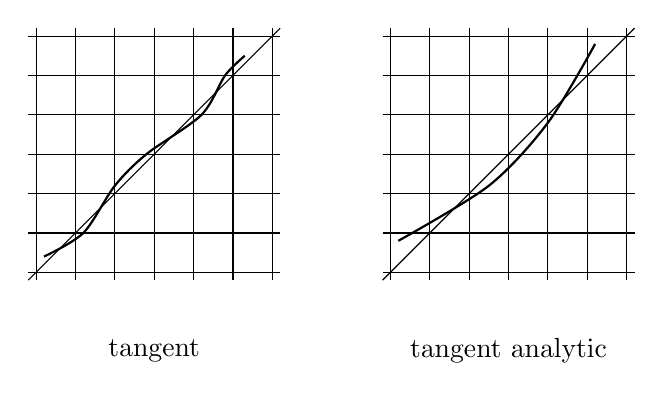
\begin{tikzpicture}[scale=0.5]
\begin{scope}[shift={(-5,0)}]
    \draw[step=1,thin] (0,0) +(-0.2,-0.2) grid +(6.2,6.2);
    \draw (-0.2,-0.2) -- (6.2,6.2);
    \draw[thick] plot[smooth,tension=.5] coordinates{(0.2,0.4) (1.2,1) (2,2.2) (2.8,3) (4.2,4) (4.8,5) (5.3,5.5)}; 
    \draw (3,-1) node {};
    \draw (3,-2) node {tangent};
\end{scope}
\begin{scope}[shift={(4,0)}]
    \draw[step=1,thin] (0,0) +(-0.2,-0.2) grid +(6.2,6.2); 
    \draw (-0.2,-0.2) -- (6.2,6.2); 
    \draw[thick] plot[smooth,tension=.5] coordinates{(0.2,0.8) (2.5,2.2) (4,3.8) (5.2,5.8) };
    \draw (3,-1) node {};
    \draw (3,-2) node {tangent analytic};
\end{scope}
\end{tikzpicture}
\end{center}





\section{Complexity}


The \emph{complexity} of a language  is the map that counts, for any
integer , the number of elements of  of length . It is usually
denoted by .
\newline
The complexity of the balanced words  was studied in
\cite{Lipatov1982}, \cite{Mignosi1991} and \cite{BerstelPocchiola1993},
where it was proved to be equal to:

where  denotes the Euler totient function: .
\newline
\newline
To compute the complexity of  and , we will use the
tools introduced by Julien Cassaigne using bispecial factors
\cite{Cassaigne1997}. They have been used in the context of billiards in
\cite{CassaigneHubertTroubetzkoy2002}.
Let  be a factorial and extendable language on the alphabet .
A word  in  is said to be \emph{bispecial} if , , , 
are in . A bispecial factor  is called 
\begin{itemize}
\item \emph{weak bispecial} if , 
\item \emph{ordinary bispecial} if ,
\item \emph{strong bispecial} if . 
\end{itemize}
Let  (resp. ) denote the number of weak (resp. strong)
bispecial factors of length  in .
Let  denote the first difference . We have:

Hence, by summing twice, if  is nontrivial, we have:

\newline
Let us first describe the combinatorial structure of bispecial factors in
.
Let  be a bispecial factor.
If  is not diagonal, then it can be desubstituted (in a single way) and
 is a bispecial factor of the same kind.
Otherwise, if  is thin diagonal, then it is strong or ordinary
bispecial depending on the parity of its length. Otherwise,  is
diagonal and the three states are visited during its recognition:  is
strong bispecial.
Hence, there is no weak bispecial factor in .
This also holds for .
\newline
\newline
The geometric characterisation of tangent (resp. tangent analytic) words
is convenient to describe and count the strong bispecial factors.
We can visualise the strong bispecial factors as follows.
Pick a segment from   to .
\newline
If there is no integer point on the way (which happens precisely when
), the coding of the corresponding open interval is a
bispecial factor of length  in both  and .
Those words are also the bispecial factors for balanced words. There are
 such words of length , this the geometrical meaning of
Lipatov's formula \cite{Lipatov1982}.
\newline \newline



\begin{center}
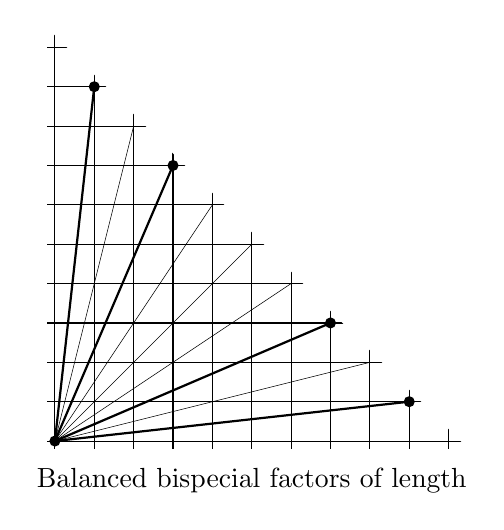
\begin{tikzpicture}[scale=0.5]
\begin{scope}[shift={(-5,0)}]
\foreach \n in {10}{
    \foreach \var in {1,3,7,9}{\draw[above right] (\var,\n-\var) node {} ;}

    \clip (-0.2,-0.2) -- (\n+0.5,-0.2) -- (-0.2,\n+0.5) -- cycle;
    \draw[step=1,thin] (0,0) +(-0.2,-0.2) grid +(\n+1,\n+1);
    \fill [black] (0,0) circle (4pt);

    \foreach \var in {1,...,\n}{
    \draw[very thin] (0,0) -- (\var,\n-\var);
    }

\foreach \var in {1,3,7,9}{
    \draw[thick] (0,0) -- (\var,\n-\var);
    \fill [black] (\var,\n-\var) circle (4pt);
    }
}

\end{scope}
\draw (0,-1) node {Balanced bispecial factors of length } ;
\end{tikzpicture}
\end{center}
Otherwise, there are  points one the way. 
For tangent analytic words, each such segment corresponds to two bispecial
factors of length : one bending above the  points, another bending under
the  points. There are  such words of length .


\begin{center}
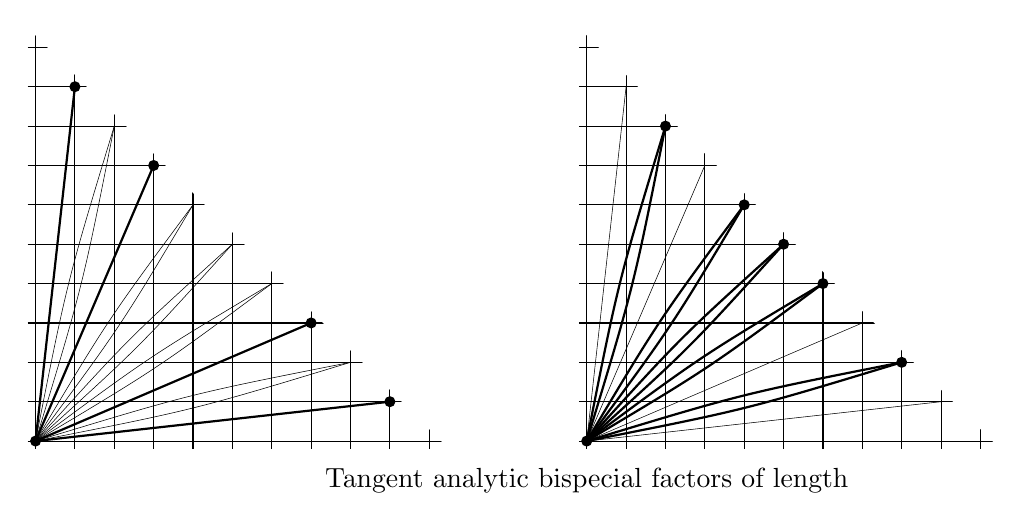
\begin{tikzpicture}[scale=0.5]


\draw (-2,5) node {\LARGE };

\begin{scope}[shift={(-14,0)}]
\foreach \n in {10}{
    \foreach \var in {1,3,7,9}{\draw[above right] (\var,\n-\var) node {} ;}

    \clip (-0.2,-0.2) -- (\n+0.5,-0.2) -- (-0.2,\n+0.5) -- cycle;
    \draw[step=1,thin] (0,0) +(-0.2,-0.2) grid +(\n+1,\n+1);
    \fill [black] (0,0) circle (4pt);

    \foreach \var in {1,3,7,9}{
    \draw[thick] (0,0) -- (\var,\n-\var);
    \fill [black] (\var,\n-\var) circle (4pt);
    }



    \foreach \var in {2,4,5,6,8}{
    \draw[very thin] (0,0) .. controls (\var/2 - \n/40 + \var/40 , \n/2 - \var/2 + \var/40)  ..  (\var,\n-\var);
    \draw[very thin] (0,0) .. controls (\var/2 + \n/40  - \var/40 , \n/2 - \var/2 - \var/40)  ..  (\var,\n-\var);
}

}
\end{scope}


\begin{scope}
\foreach \n in {10}{
    \foreach \var in {2,4,5,6,8}{\draw[above right] (\var,\n-\var) node {} ;}

    \clip (-0.2,-0.2) -- (\n+0.5,-0.2) -- (-0.2,\n+0.5) -- cycle;
    \draw[step=1,thin] (0,0) +(-0.2,-0.2) grid +(\n+1,\n+1);
    \fill [black] (0,0) circle (4pt);

    \foreach \var in {1,3,7,9}{
    \draw[very thin] (0,0) -- (\var,\n-\var);
    }



    \foreach \var in {2,4,5,6,8}{
    \draw[thick] (0,0) .. controls (\var/2 - \n/40 + \var/40 , \n/2 - \var/2 + \var/40)  ..  (\var,\n-\var);
    \draw[thick] (0,0) .. controls (\var/2 + \n/40  - \var/40 , \n/2 - \var/2 - \var/40)  ..  (\var,\n-\var);
\fill [black] (\var,\n-\var) circle (4pt);
    }

}
\end{scope}


\draw (0,-1) node {Tangent analytic bispecial factors of length } ;
\end{tikzpicture}
\end{center}
For tangent words, each such segment corresponds to  bispecial
factors of length  corresponding to all the possibilities of
slaloming around the  integer points on the way. 
Hence, there are  strong bispecial factors of length  in
.




\begin{center}
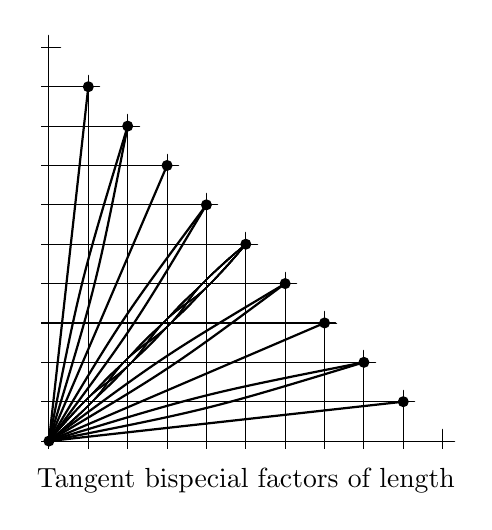
\begin{tikzpicture}[scale=0.5]

\begin{scope}[shift={(-5,0)}]
\foreach \n in {10}{

    \foreach \var in {1,3,7,9}{\draw[above right] (\var,\n-\var) node {} ;}
    \foreach \var in {2,4,6,8}{\draw[above right] (\var,\n-\var) node {} ;}
    \draw[above right] (\n/2,\n/2) node {} ;

    \clip (-0.2,-0.2) -- (\n+0.5,-0.2) -- (-0.2,\n+0.5) -- cycle;
    \draw[step=1,thin] (0,0) +(-0.2,-0.2) grid +(\n+1,\n+1);
    \fill [black] (0,0) circle (4pt);

    \foreach \var in {1,3,7,9}{
    \draw[thick] (0,0) -- (\var,\n-\var);
    \fill [black] (\var,\n-\var) circle (4pt);
    }



    \foreach \var in {2,4,6,8}{
    \draw[thick] (0,0) .. controls (\var/2 - \n/40 + \var/40 , \n/2 - \var/2 + \var/40)  ..  (\var,\n-\var);
    \draw[thick] (0,0) .. controls (\var/2 + \n/40  - \var/40 , \n/2 - \var/2 - \var/40)  ..  (\var,\n-\var);
\fill [black] (\var,\n-\var) circle (4pt);
    }
    \foreach \i in {-1,1}{
        \foreach \j in {-1,1}{
            \foreach \k in {-1,1}{
                \foreach \l in {-1,1}{
                    \draw[-] plot[smooth,tension=0.9] coordinates{(0,0)
(1+\i/20,1-\i/20) (2+\j/20,2-\j/20) (3+\k/20,3-\k/20) (4+\l/20,4-\l/20)
(\n/2,\n/2)};


    }
    }        
    }
    }

    \fill [black] (\n/2,\n/2) circle (4pt);

}
\end{scope}


\draw (0,-1) node {Tangent bispecial factors of length } ;
\end{tikzpicture}

\end{center}






\begin{proposition}
We have:





\end{proposition}




\section{Conclusion}

Let us recall that a word  is -\emph{balanced} if:




Each class of words is strictly included in the next one:
\begin{itemize}
\item -balanced words (digital straight segments)
\item tangent analytic words
\item tangent words
\item -balanced words \\
\end{itemize}
The complexity of the first two classes, is cubical whereas the complexity
of the last two classes is exponential.
It can be shown that analytic tangent words can be written as a
concatenation of two -balanced words. What is the gap between tangent
words and -balanced words ?


\bibliographystyle{eptcs}
\bibliography{biblio}

\end{document}
